\section{Motivation}
\label{ch:introduction:motivation}
Sound systems are used world wide to fill rooms with enjoyable audio content. 
Problems arise however when multiple people in the same room want to enjoy different audio content at the same time.

For example, one person may want to enjoy a show, while an other may want to listen to their music.
If they are in the same room, their desires clash: neither person can fully enjoy their chosen activity without disturbing
the other.
In short, the interference of multiple source of audio leads to a situation where both individual experiences are diminished.

In recent years, attempts have been made to solve this problem by controlling the spatial reproduction of sound in such
a way that different areas in a room have different sound content.

One class of algorithms that attempt to do so are known as sound zone algorithms~\cite{betlehem2015personal}.
Sound zone algorithms partition the space of the room into multiple so-called sound zones.
Each sound zone is assigned different audio content.

The sound zone algorithms decides how to use the sound system to reproduce audio content in each zone.
Using the principals of constructive and destructive interference, this is done in such a way that minimal 
content of one zone is audible in the others.

In the previously listed example, one zone would contain the audio of a show and another zone would contain music.
The sound zone algorithm would then determine how to best use the sound system to reproduce the two zones.
If the sound zone algorithm does a good job, both people can enjoy their audio content at its full potential 
without bothering one another.
An image depicting the situation is given in \autoref{fig:introduction:motivation:concept}.

\begin{figure}[t]
    \centering
    \scalebox{1.0}{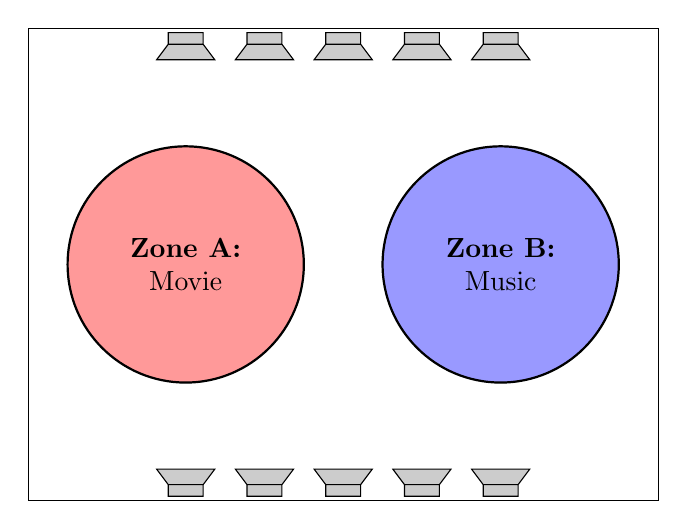
\begin{tikzpicture}
    \tikzset{
      Speaker/.pic={
        \filldraw[fill=gray!40,pic actions] 
        (-15pt,0) -- 
          coordinate[midway] (-front) 
        (15pt,0) -- 
        ++([shift={(-6pt,8pt)}]0pt,0pt) coordinate (aux1) -- 
        ++(-18pt,0) coordinate (aux2) 
        -- cycle 
        (aux1) -- ++(0,6pt) -- coordinate[midway] (-back) ++(-18pt,0) -- (aux2);
      }
    }

    \draw [draw=black] (0,0) rectangle (8,6);

    % Speakers on the top wall
    \pic[scale=0.7] at (2, 5.6) {Speaker};
    \pic[scale=0.7] at (3, 5.6) {Speaker};
    \pic[scale=0.7] at (4, 5.6) {Speaker};
    \pic[scale=0.7] at (5, 5.6) {Speaker};
    \pic[scale=0.7] at (6, 5.6) {Speaker};

    % Speakers on the bottom wall
    \pic[rotate=180, scale=0.7] at (2, 0.4) {Speaker};
    \pic[rotate=180, scale=0.7] at (3, 0.4) {Speaker};
    \pic[rotate=180, scale=0.7] at (4, 0.4) {Speaker};
    \pic[rotate=180, scale=0.7] at (5, 0.4) {Speaker};
    \pic[rotate=180, scale=0.7] at (6, 0.4) {Speaker};

    \draw[opacity=0.4, fill=blue] (6,3) circle[radius=1.5];
    \draw[thick] (6,3) circle (1.5) node[align=center] {\textbf{Zone B:}\\Music};
    \draw[opacity=0.4, fill=red]  (2,3) circle[radius=1.5];
    \draw[thick] (2,3) circle (1.5) node[align=center] {\textbf{Zone A:}\\Movie};
\end{tikzpicture}
}
    \caption{A room containing a sound system consisting of an array of loudspeakers and two zones.
                The goal of the sound zone algorithm is to control the sound system in such a way that the red zone
                contains the audio of a show, and the blue zone contains the music.}
    \label{fig:introduction:motivation:concept}
\end{figure}

In practice however, sound zone algorithms do not always do a perfect job.

The performance of algorithms depends on the environment and the available sound system.
Depending on the situation, the interference between zones can typically only be reduced by so much.
As such, audio content of one zone is often still audible in other zones.
In addition to this, reducing interference between zones can also come at the cost of reducing quality of the 
reproduced audio in the zones.

Improving sound zone algorithms is still an active topic of research.
One recent approach is to include a model of the human auditory system to model how sound is perceived.
Typically, sound zone algorithms model physical quantities such as sound pressure, which doesn't always capture
what is important for the perception of sound.
As such, including a perceptual model may allow the algorithm to focus on the parts of the audio content
that matter perceptually.

Early results show that the perceptual sound zone approach is promising.
Recent work by Donley et al. explored including the absolute threshold of hearing, which models the lowest sound pressure
humans can hear, into sound zone algorithms.
In this pursuit it was found that the quality of the reproduced audio in the zones~\cite{donley2015multizone}.
Later, Lee et al. showed that including a perceptually-motivated weighting in the sound zone algorithm outperforms 
traditional algorithms~\cite{lee2019towards,lee2020signal}.

This work will seek to further explore this perceptual approach by proposing a novel perceptual sound zone algorithm.
A perceptual sound zone algorithm will be constructed from scratch by considering what perceptual models and sound
zone algorithms are best suited to integrate into one another.
